
\documentclass[11pt,a4paper,slovene]{myarticle}

%Uporabljeni paketi
\usepackage[slovene]{babel}
\usepackage[utf8]{inputenc}
\usepackage{lmodern}
\usepackage[T1]{fontenc}
\usepackage{fancyhdr}
\usepackage{caption}
\captionsetup{font={default,footnotesize}, labelfont=bf, format=hang,indention=.0cm}
\usepackage{graphicx,epsfig}
\usepackage{amsmath}
\usepackage{multirow}
\usepackage{color}
\usepackage{url}
\usepackage{makeidx}
\usepackage{listings}
\usepackage[official]{eurosym}

\definecolor{dkgreen}{rgb}{0,0.6,0}
\definecolor{gray}{rgb}{0.5,0.5,0.5}
\definecolor{mauve}{rgb}{0.58,0,0.82}

\lstset{frame=tb,
  language=C++,
  aboveskip=3mm,
  belowskip=3mm,
  showstringspaces=false,
  columns=flexible,
  basicstyle={\small\ttfamily},
  numbers=none,
  numberstyle=\tiny\color{gray},
  keywordstyle=\color{blue},
  commentstyle=\color{dkgreen},
  stringstyle=\color{mauve},
  breaklines=true,
  breakatwhitespace=true,
  tabsize=3
}

\usepackage{hyperref}
\hypersetup{
   bookmarksnumbered=true,
   urlbordercolor={0 1 0},
   linkbordercolor={1 1 1},
   unicode=true,
   pdftitle={ Modeliranje Računalniških Omrežij },
   pdfauthor={Asistent},
   pdfdisplaydoctitle=true,
   pdftoolbar=true,
   pdfmenubar=true,
   pdfstartview=X Y Z
}

\urlstyle{same}

\setlength{\parskip}{12pt}
\setlength\parindent{0pt}
\setlength\unitlength{1mm}

\begin{document}
\label{naslov}
\pdfbookmark[1]{Naslov}{naslov}
\thispagestyle{empty}

\begin{center}
\begin{Large}
Modeliranje računalniških omrežij\\
Študijsko leto 2019/2020\\
\end{Large}

\vspace*{4cm}
\begin{LARGE}
\textbf{Naloga 4 - Modeliranje IPv6 omrežij\\}
\end{LARGE}
\vspace*{0.5cm}

\begin{Large}
Poročilo za drugo seminarsko nalogo\\

\vspace*{4cm}

Mihael Šinkec\\
Vpisna št. 63170277\\
Matej Fortuna\\
Vpisna št. 63170091\\
Matej Fajdiga\\
Vpisna št. 63170084\\
Dominik Skapin\\
Vpisna št. 63150262\\

\vspace*{2cm}
Ljubljana, \today
\end{Large}
\end{center}

\pagebreak
\setcounter{page}{1}
\pagenumbering{arabic}


\label{Kazalo}
\pdfbookmark[1]{Kazalo}{Kazalo}
\tableofcontents
\thispagestyle{empty}
\pagebreak

\section{Opis primerov IPv6 omrežij}
\subsection{Omrežje 1 - IPv6 N Clients}
To omrežje je sestavljeno iz odjemalca, strežnika in treh IPv6 usmerjevalnikov. Strežnik nudi dostop s telnet protokolom, preko katerega odjemalec dostopa nanj.

\begin{figure}[h]
  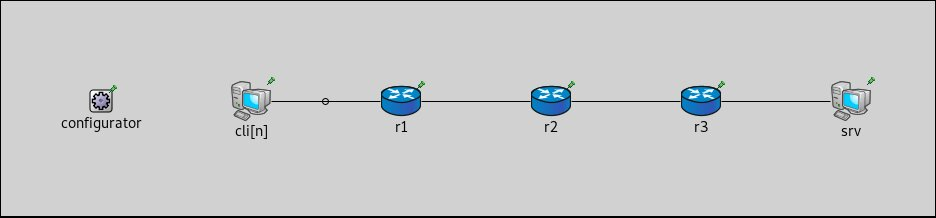
\includegraphics[width=\linewidth]{ipv6nclients.jpg}
\end{figure}

Povezave (na 2. nivoju po TCP/IP) med posameznimi napravami se lahko nastavijo na Ethernet oz. na PPP protokol.

\subsection{Omrežje 2 - IPv6 Bulk Transfer}
Tukaj piši, Matej, in zavrti kolo.......


\end{document}











